\documentclass[]{rsuqbeamernew}


\title[UQWorld]{UQWorld: an Applied UQ Community}

\author[D. Wicaksono]{Damar Wicaksono}
\institute[RSUQ, ETH Z\"urich]{Chair of Risk, Safety and Uncertainty 
Quantification -- ETH Z\"urich}

\date[09.05.2019]

\graphicspath{{Figures/}}
\usepackage{caption}
\usepackage{listings}
\usepackage{tikz}
\usepackage{pifont}
\usepackage{booktabs}% http://ctan.org/pkg/booktabs
\newcommand{\tabitem}{~~\llap{\textbullet}~~}
%\def\checkmark{\tikz\fill[scale=0.4](0,.35) -- (.25,0) -- (1,.7) -- (.25,.15) -- cycle;}

%% Note: the title page will be created automatically



\begin{document}

%===============================================================================
\begin{frame}{Outline}

\tableofcontents

\end{frame}
%===============================================================================

\section{UQLab Users}

%===============================================================================
\begin{frame}{Background}

We tried to get some ideas for our UQ community based on
our understanding of the \emph{apparent} audience, i.e., \textbf{UQLab users}: 

\begin{itemize}
  \item Since its public release in 2015, UQLab users has almost reached 2'000 users from 77 countries,
  with over 60 unique active users per day and up to 130 weekly.
  \item We ask users to register, but beyond users affiliation,
  we don't know much about them or how they are using UQLab\footnote{Which are not the point of registration.
  For the actual reasons on why registration is required,
  see Stefano's blog on \emph{Why a licensing system? Is UQLab really open source?}
  in \texttt{UQWorld}}.
\end{itemize}

How can we know more of our audience, up to the present?

% Ideas mean who is for, what is it about
\end{frame}
%===============================================================================

%===============================================================================
\begin{frame}{UQLab users: A glimpse from support emails}

Many are about registration, installations, and license:

\begin{itemize}
  \item From:$\blacksquare@\blacksquare$.com, Subject: Registration, captcha
    \begin{quotation}
      Trying to register for downloading UQLab, I always fail to find the captcha.
      Could you please check it? I'd be surprised to find out that I am a bot :)
    \end{quotation}
  
  \item From:$\blacksquare.\blacksquare@\blacksquare$.edu, Subject: problem while installing uqlab
    \begin{quotation}
      i have problems installing on MATLAB 2010b, the version 2014a seems to work ok. i just want to let you know about that. 
    \end{quotation}

  \item From:$\blacksquare@\blacksquare$.fr, Subject: Loose the licence file
    \begin{quotation}
      I'm PhD candidate and I want to use your UQlab toolbox but I loose my licence email and I can't find it on my computer.
    \end{quotation}
    
\end{itemize}

\end{frame}
%===============================================================================

%===============================================================================
\begin{frame}{UQLab users: A glimpse from support emails}
  
  Some are technical questions about UQLab:
  \begin{itemize}
    \item From:$\blacksquare@\blacksquare$.edu.au, Subject: sequential design strategy
    \begin{quotation}
      However I was wondering if there is a way to set up sequential design strategy in UQlab. 
    \end{quotation}
    \item From: many, Subject: Problem with running UQlab
    \begin{quotation}
      I am running this piece of code:
      ....
      and am seeing this error message:
      ....
      I was wondering if you had any suggestions to resolving this problem.
    \end{quotation}
  \end{itemize}

  Some are technical questions about UQ in practice (and in context):
  \begin{itemize}
      \item From:$\blacksquare@\blacksquare$.ch, Subject: Best case and worst case during uncertainity quantification
      \begin{quotation}
      Lately our group is trying to use Monte Carlo approach to quantify uncertainty in our estimation of human optimum walking performance.
      Particularly, we require some knowledge on defining the best and worst case scenarios.
      Can you guide us ? 
    \end{quotation}
  \end{itemize}


\end{frame}
%===============================================================================

%===============================================================================
\begin{frame}{UQLab users: A glimpse from support emails}

Some are nice,
\begin{itemize}
  \item From: $\blacksquare@\blacksquare$.de, Subject: Citing UQLab
  \begin{quotation}
    As I won't have the chance to employ it in my work, \textbf{I would like to include it in my literature section to raise awareness for students after me}.
    Unfortunately, I couldn't find how to cite UQLab. Any recommendations?
  \end{quotation}
  \item From: $\blacksquare@\blacksquare$.pt, Subject: credits in publications
  \begin{quotation}
    \textbf{I haven't started to use UQlab yet} but at a glance \textbf{let me tell you that it seems a very nice job!}
  \end{quotation}
\end{itemize}

Some can be nicer...
\begin{itemize}
  \item From:$\blacksquare@\blacksquare$.edu, Subject: Unregister
  \begin{quotation}
    Kindly cancel my registration!
    
    Thank you!
  \end{quotation}
\end{itemize}

\end{frame}
%===============================================================================

%===============================================================================
\begin{frame}{UQLab users: A glimpse from support emails}

Some are a bit hard to read,
\begin{itemize}
  \item From: $\blacksquare@\blacksquare$.edu.cn, Subject: Matlab code by Dr. Moustapha w.r.t. the fascinating Quantile-based RBDO
  \begin{quotation}
    Good dinner Dr. Moustapha \\
    Your catchy Quantile-based RBDO bring up new ideas for our RBDO world.
    If Dr. Moustapha is going to need allies or assistants for your idea to gain momentum, sincere hope for good cooperation (fans) between us (of yours) \texttt{\textasciitilde.\textasciitilde}!
    Actually, me is a current Master student w.r.t. Reliabil \& Syst Engn.
    If I make the decision to embark on a PhD, your QB-RBDO is really fascinating for me.(Wow! Such a productve and effective methodology for practical applications.That's terrific!)
  \end{quotation}
\end{itemize}

\end{frame}
%===============================================================================

%===============================================================================
\begin{frame}[t]{UQLab users: A glimpse from external citations}

\begin{columns}
    \column{0.5\textwidth}
  \begin{minipage}[c][0.30\textheight][c]{\linewidth}
    \begin{figure}
      \centering
      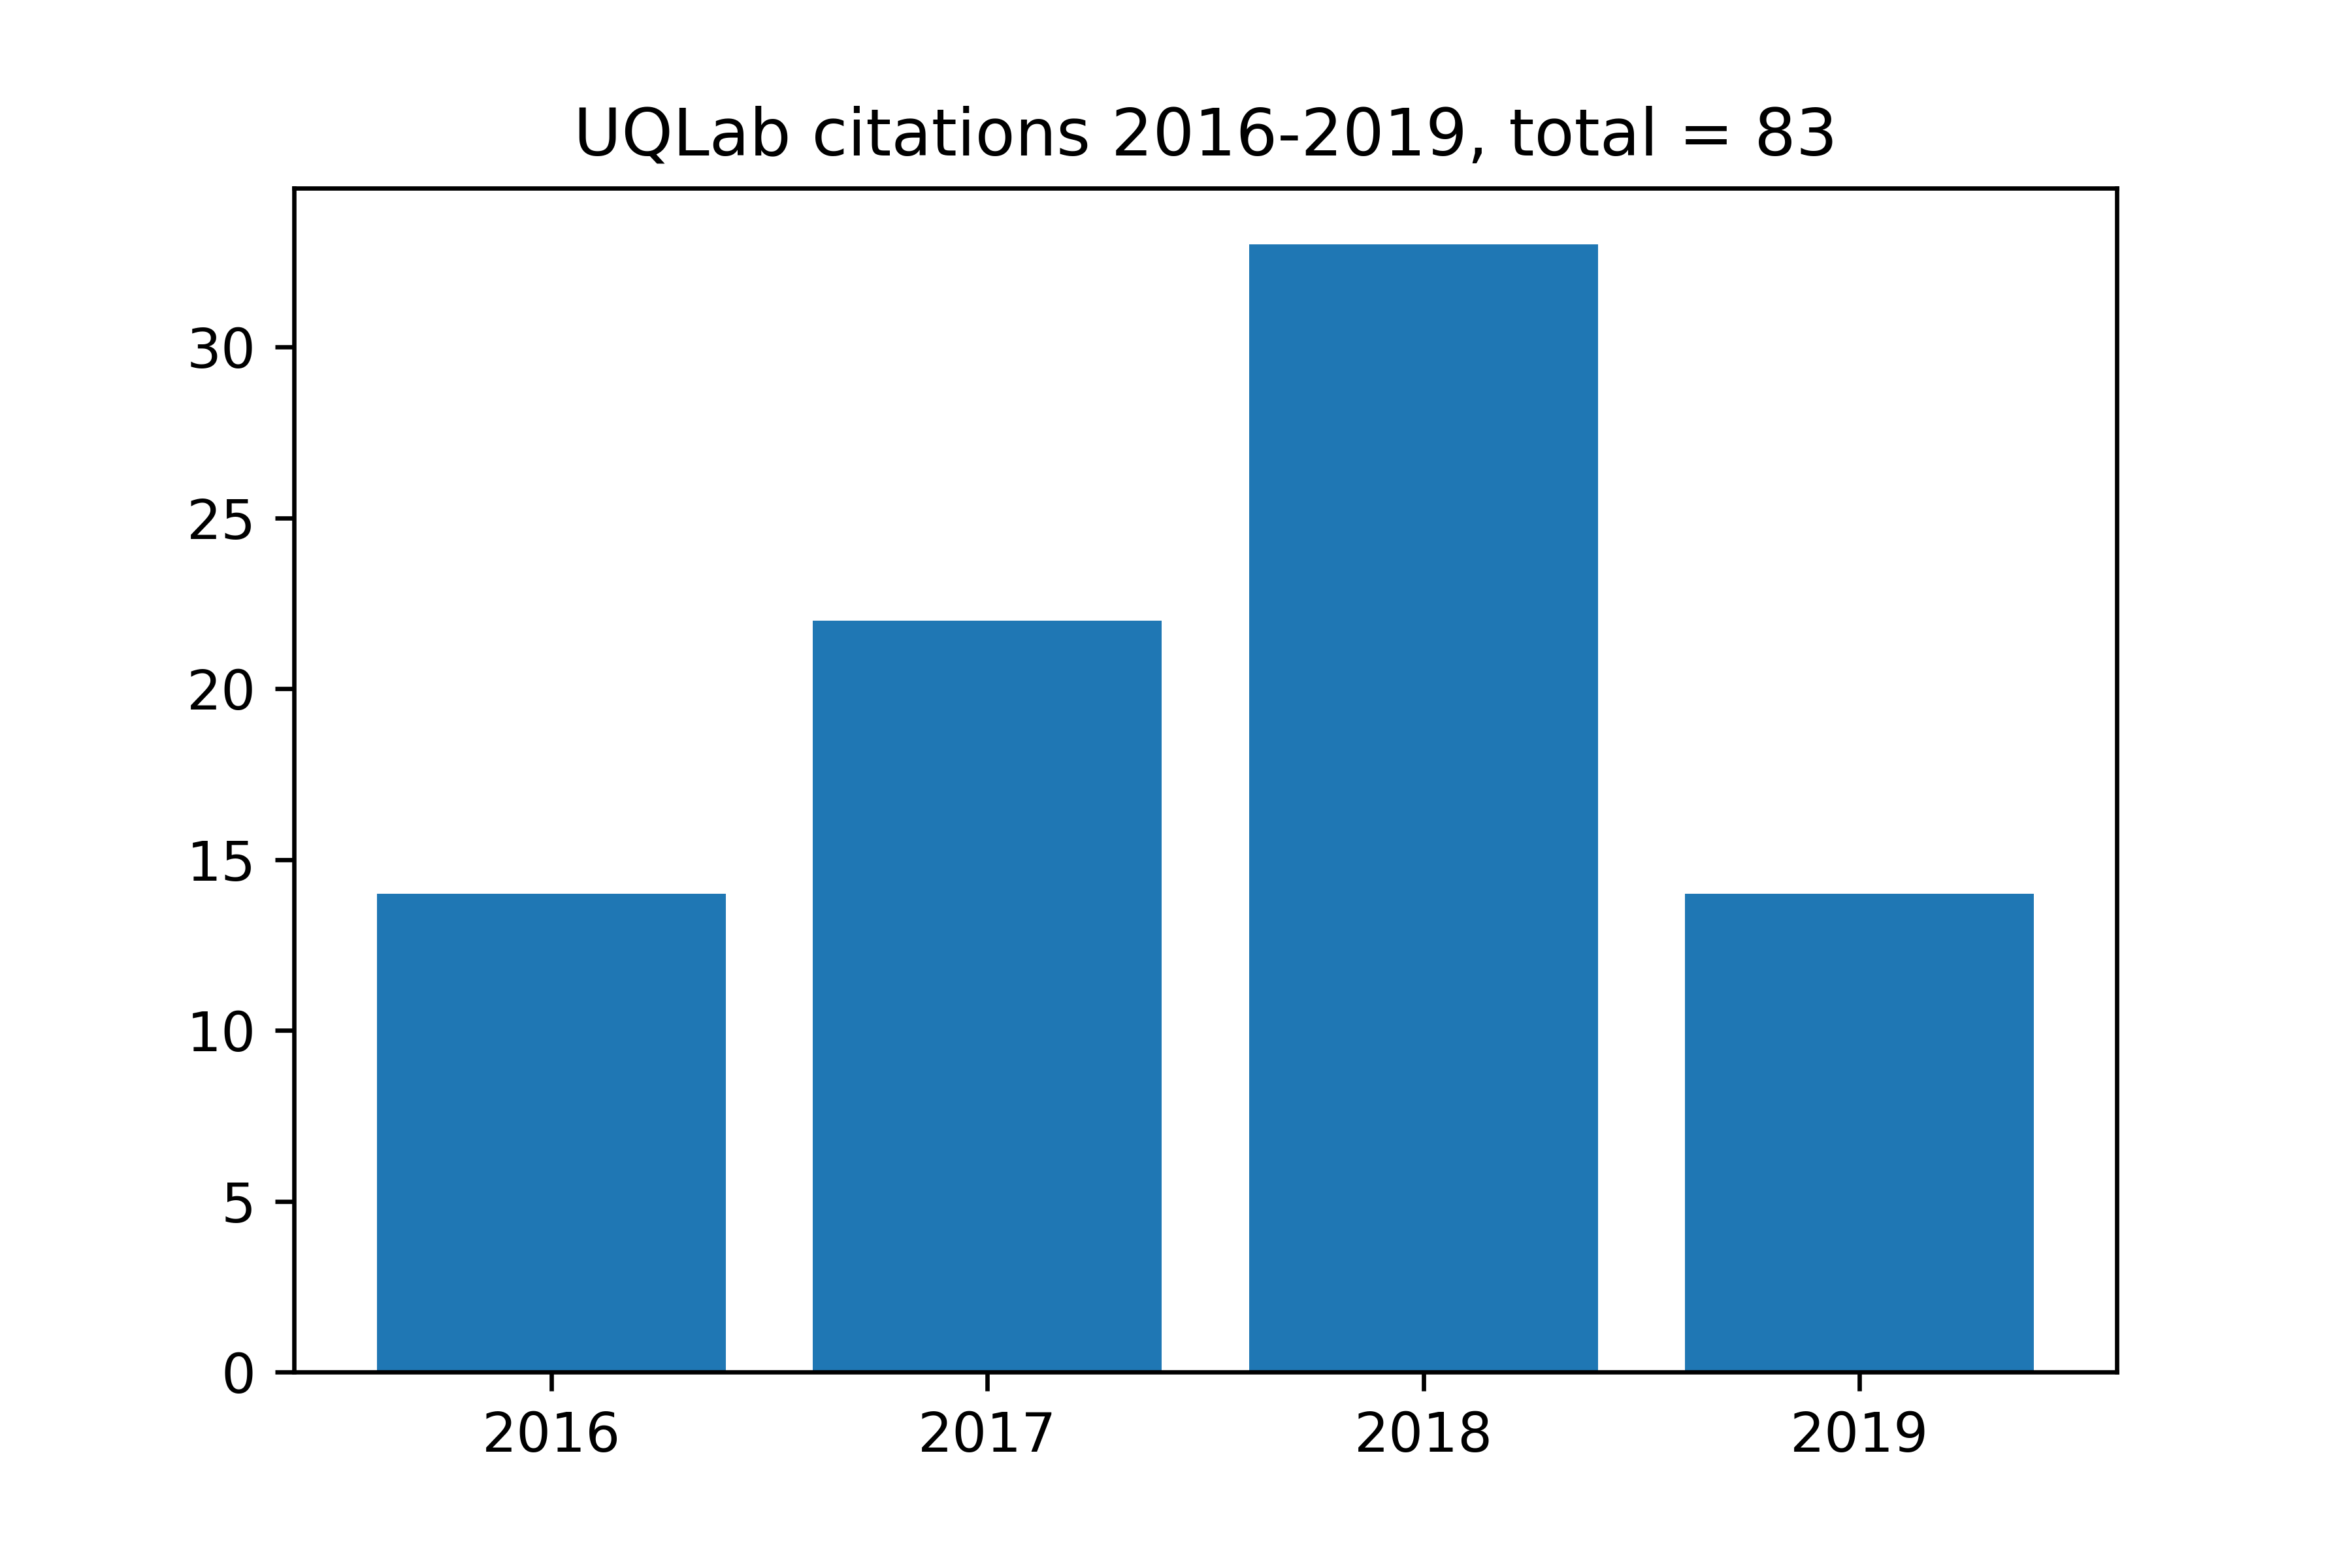
\includegraphics[width=0.8\linewidth]{../figures/cit_stat}
    \end{figure}
  \end{minipage}
  \begin{minipage}[c][0.6\textheight][c]{\linewidth}
    \begin{figure}
      \centering
      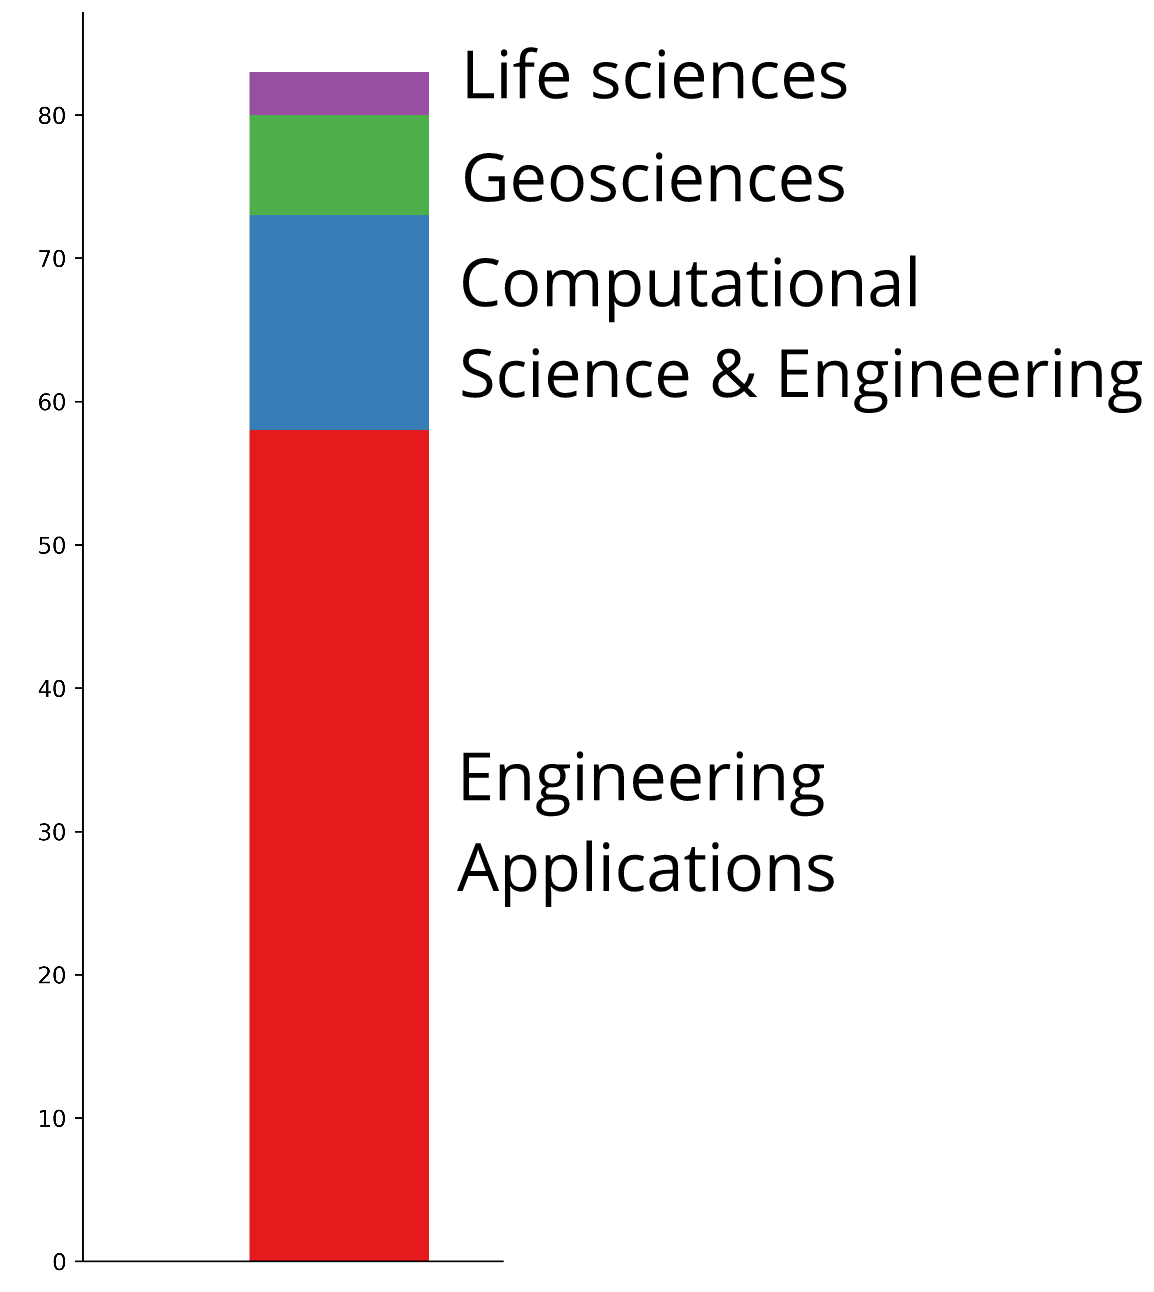
\includegraphics[width=0.75\linewidth]{../figures/uqlab_citations}
    \end{figure}
  \end{minipage}

  \column{0.5\textwidth}
    \begin{itemize}
    \item Between 2016--2019, about 83 papers are published in which UQLab is used as an analysis tool.
    \item \emph{Engineering applications} is the majority.
  \end{itemize}
  \begin{minipage}{\linewidth}
    \begin{tabularx}{\textwidth}{Xc}
      \hline
      \scriptsize{Fields of Applications} & \footnotesize{Number of Citations} \\
      \hline
      \footnotesize{Electrical} & 19  \\
      \footnotesize{Civil} & 11 \\
      \footnotesize{Chemical} & 7 \\
      \footnotesize{Mechanical} & 6 \\
      \footnotesize{Remote sensing} & 5 \\
      \footnotesize{Nuclear} & 5 \\
      \footnotesize{Ocean} & 4 \\
      \footnotesize{Energy} & 1 \\
      \hline
    \end{tabularx}
  \end{minipage}%
  \hfill
\end{columns}

\end{frame}
%===============================================================================

%===============================================================================
\begin{frame}[t]{UQLab users: Some can be very productive}
  
Some authors are able to produce multiple papers using UQLab as part of their analysis.
For example:

  \begin{thebibliography}{Dijkstra, 1982}
    \footnotesize{
    \bibitem[Xie and Schenkendorf, 2019]{Xie2019}
    Xiangzhong Xie and Ren\'e Schenkendorf,
    \newblock Stochastic back-off-based robust process design for continuous crystallization of ibuprofen, {\em Computers and Chemical Engineering}, 2019.
    
    \bibitem[Xie et al., 2018]{Xie2018}
    Xiangzhong Xie, R\"udiger Ohs, A. C. Spiess, Ulrike Krewer, and Ren\'e Schenkendorf,
    \newblock Moment-independent sensitivity analysis of enzyme-catalyzed reactions with correlated model parameters, {\em IFAC-PapersOnLine}, 2018.
    
    \bibitem[Emenike, 2017]{Emenike2018}
    V. N. Emenike, Xiangzhong Xie, Ren\'e Schenkendorf, A. C. Spiess, and Ulrike Krewer,
    \newblock Robust dynamic optimization of enzyme-catalized carboligation: a point estimate-based back-off approach, {\em Computers and Chemical Engineering}, 2018.
  
    \bibitem[Schenkendorf et al., 2017]{Schenkendorf2017}
    Ren\'e Schenkendorf, Xiangzhong Xie, and Ulrike Krewer,
    \newblock An efficient polynomial chaos expansion strategy for active fault identification of chemical processes, {\em Computer Aided Chemical Engineering}, 2017.

    \bibitem[Xie et al., 2017]{Xie2017}
    Xiangzhong Xie, Ren\'e Schenkendorf, and Ulrike Krewer,
    \newblock Robust design of chemical processes based on a one-shot sparse polynomial chaos expansion concept, {\em Computer Aided Chemical Engineering}, 2017.}
  \end{thebibliography}
% Note that there are other cases
\end{frame}
%===============================================================================

\section{Ideas for an Online Community}

%===============================================================================
\begin{frame}[t]{Ideas for an Online Community}

% Users need help, they might demand something, and some are ready to give back.
% Audience from users is readily available (_you build it, and they will come_).
Many user online communities started as support communities, but if \emph{only} for that:
\begin{itemize}
  \item it'll be too restrictive % If UQ is somehow already a niche, then UQLab users would even be smaller bunch of audience. We attached too much the growth of the community with the growth of UQLab. Finally, there are times that you yourself would be more interested talking about UQ than just UQLab.
  \item it's not very aspiring
\end{itemize}

\vspace{0.3cm}

Widening the scope to applied UQ makes sense as there's potential audience wider than UQLab users\footnote{not to mention it fits this sentence: \emph{It promotes an active collaboration with research groups in ETH and in other universities in order to disseminate the good practices and associated tools for uncertainty quantification}. UQLab is not a pre-requisite.}.
%in context
\vspace{0.3cm}

Besides, there seems to be an opportunity...

% Makes sense because it also fits with the Chair's mission:
% It promotes an active collaboration with research groups in ETH and in other universities in order to disseminate the good practices and associated tools for uncertainty quantification. UQLab is not a pre-requisite.
\end{frame}
%===============================================================================

%===============================================================================
\begin{frame}[t]{Other UQ Online Communities?}

\begin{columns}
  \column{0.5\textwidth}
  \begin{figure}
    
\includegraphics[width=0.70\textwidth]{../figures/dakota}
  \end{figure}
  
  \column{0.5\textwidth}
  \begin{figure}
    
\includegraphics[width=0.45\textwidth]{../figures/openTurns}
  \end{figure}
\end{columns}

\begin{itemize}
  \item Dakota maintains mailing lists,
        but this is 2019\footnote{not that mailing list has become obsolete, but it definitely has its downsides for (starting) a community.}.
  \item OpenTurns maintains a blog, or not (last post July 2018, peak posts 2011, no public discussions). 
  \item Otherwise, zero relevant results from Google search
        for ``uncertainty quantification community'' or ``uncertainty quantification forum''.
\end{itemize}

\end{frame}
%===============================================================================

%===============================================================================
\begin{frame}[t]{A (long) sentence for a UQ online community}

We aim our UQ online community to be a community of:

\begin{itemize}
  \item UQ practitioners and researchers, and
  \item UQLab users
\end{itemize}

across different level of expertise---from the unitiated to experts---to:

\begin{itemize}
  \item learn the basics as well as new things in UQ;
  \item discuss UQ-related topics, share news, knowledge and experience, and showcase expertise;
  \item get and give help in using UQLab and discuss UQLab features and its continuous development.
\end{itemize}

%such that it becomes:
%\begin{itemize}
%  \item the definitive place to discuss and share online topics related to UQ;
%  \item the home for UQLab users (incl., at some point, external contributors) online community.
%\end{itemize}

%\begin{tabularx}{\textwidth}{XX}
%  \hline
%  Questions                            & Answers \\
%  \hline
%  \emph{What will the community be about?}               & About UQ and UQLab-related topics \\
%  \emph{Who is the community for?}                       & UQ practitioners, researchers, and UQLab users \\
  
%  \emph{What is the purpose or goal of the community? What UQLab community strive for?}
%  & \tabitem Be a place to discuss about, share, learn, and get help in topics related to UQ, from beginners to advanced \\
%  & \tabitem Be the definitive community-powered home for UQLab support and best practices \\
  
%  \emph{What will happen in the community?}          & Selection of various contents (editorial and user-generated), free form discussion, knowledge base \\
  

%  \hline
%\end{tabularx}

\end{frame}
%===============================================================================

\section{Tools for an Online Community}

%===============================================================================
\begin{frame}[t]{Tools for an Online Community}

  \begin{columns}
    \column{0.50\textwidth}
    \begin{minipage}[c][0.80\textheight][c]{\linewidth}
      \begin{figure}
        \centering
        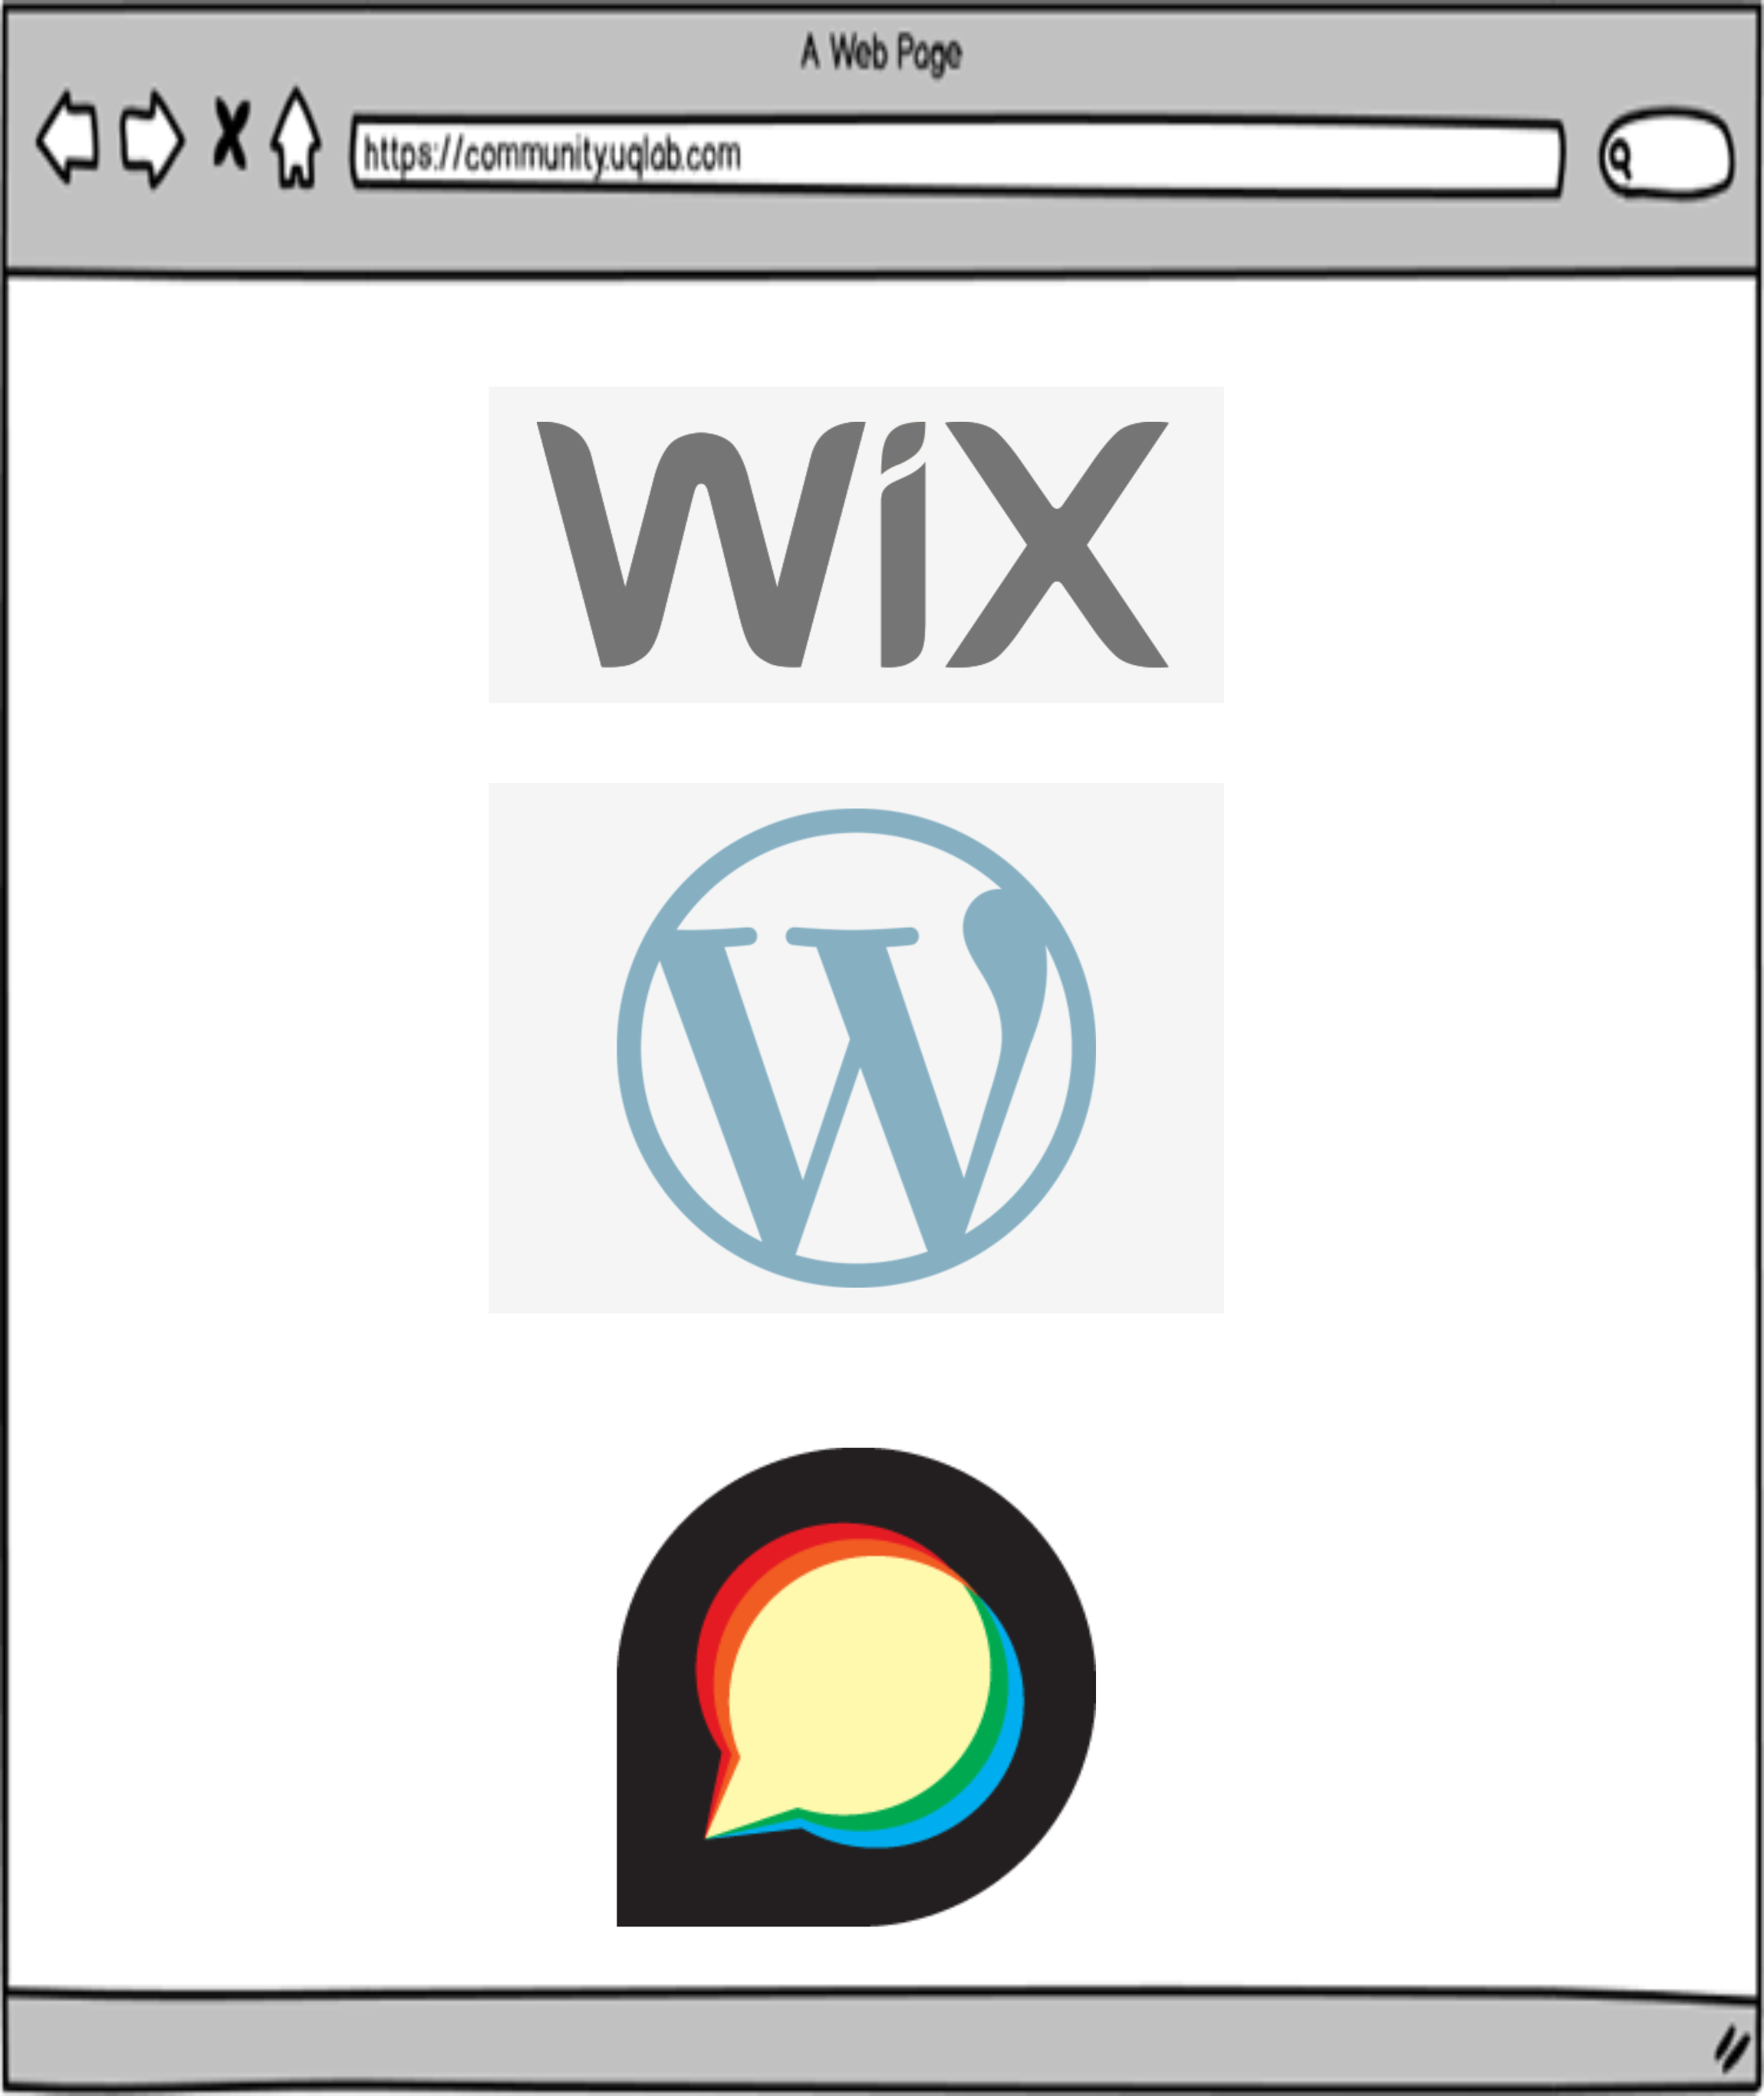
\includegraphics[width=1.0\linewidth]{../figures/communityPlatform}
      \end{figure}
    \end{minipage}
      
    \column{0.50\textwidth}
    Three possible platforms or tools were considered:
  \begin{itemize}
    \item Wix: What we already have (\texttt{uqlab.com}) plus a forum plugin.
    \item Wordpress: Entirely new website (\textbf{a blog, with a forum} plugin).
    \item Discourse: Entirely new website (\textbf{a forum, with some kind of blog}).
  \end{itemize}
  We decided to go on with Discourse. % Because of relative simplicity, more out-of-the-box modern forum, lower bar of participation, great search functionalities. In Wordpress, so much thinkering in the forum plugin to have it on par with more modern forum. It's about the amount of tinkering we want.
  \hfill
  
 \end{columns}
% mainly forum plus some (limited) customization for blogs
\end{frame}
  
\section{UQWorld (with Demo)}

%===============================================================================
\begin{frame}[t]{Introducing UQWorld}
  
  \begin{columns}
    \column{0.30\textwidth}
    \begin{minipage}[c][0.85\textheight][c]{\linewidth}
      \begin{figure}
        \centering
        
\includegraphics[width=1.0\linewidth]{../figures/uqworld_logo.png}
      \end{figure}
    \end{minipage}
      
    \column{0.70\textwidth}
    \begin{itemize}
      \item An online community platform for applied UQ.
      \item Already live (but not public) at \texttt{uqworld.org}.
      \item Will be open to all: exploration (browsing) is public,
            but any participation requires registration.
      \item Three main categories: 
      \begin{itemize}
        \item Learn and discuss UQ topics (\emph{All About UQ})
        \item News, updates, case studies, other community resources, and meta-discussion (\emph{UQ Resources})
        \item UQLab support \& Development (\emph{UQ with UQLab})
      \end{itemize}
    \end{itemize}
    \hfill
    \begin{columns}
      \column{0.3\textwidth}
      \begin{figure}
        
\includegraphics[width=0.70\textwidth]{../figures/all-about-uq_512}
        \caption*{All About UQ}
      \end{figure}
      
      \column{0.3\textwidth}
      \begin{figure}
        
\includegraphics[width=0.65\textwidth]{../figures/uq-resources_512}
        \caption*{UQ Resources}
      \end{figure}
      
      \column{0.3\textwidth}
      \begin{figure}
        
\includegraphics[width=0.6\textwidth]{../figures/uq_with_uqlab_512}
        \caption*{UQ with UQLab}
      \end{figure}
    \end{columns}
  \end{columns}

\end{frame}
%===============================================================================

%===============================================================================
%\begin{frame}[t]{UQWorld: Structure and organization}
  
%\texttt{UQWorld} is organized into three main categories:
%\begin{columns}
 % \column{0.3\textwidth}
  %\begin{figure}
   % 
\includegraphics[width=0.70\textwidth]{../figures/all-about-uq_512}
   % \caption*{All About UQ}
  %\end{figure}
  
 % \column{0.3\textwidth}
 % \begin{figure}
 %   
\includegraphics[width=0.65\textwidth]{../figures/uq-resources_512}
 %   \caption*{UQ Resources}
 % \end{figure}
  
 % \column{0.3\textwidth}
 % \begin{figure}
 %   
\includegraphics[width=0.6\textwidth]{../figures/uq_with_uqlab_512}
 %   \caption*{UQ with UQLab}
 % \end{figure}
%\end{columns}

%\begin{itemize}
  %\item \emph{All About UQ} contains the free UQ discussion forum and the Chair's published post (\textbf{UQ-centered} space).
  %\item \emph{UQ Resources} contains news, updates, case studies, and other resources from UQ community at large (\textbf{UQ-centered} space).
  %\item \emph{UQ with UQLab} is the corner for UQLab users, a place to get help with UQLab, as well as updates from the Developer Team (\textbf{UQLab-centered} space).
%\end{itemize}

%\end{frame}
%===============================================================================

%===============================================================================
%\begin{frame}[t]{UQWorld: An Applied UQ Community}
  
%The largest chunk of space in \texttt{UQWorld} caters to UQ practitioners---from the uninitiated to experts---regardless the software tool they are using:

%\begin{itemize}
%  \item \emph{UQ Discussion Forum}: A lightly-moderated forum to ask, discuss, and share (Examples: Introduce projects and UQ methods applied, )
%  \item \emph{Chair's Blog} (Example: Bruno's posts on \emph{Getting started with UQ} and \emph{How to define my probabilistic input distributions?}).
%  \item \emph{News and Announcements} (Example: Paul's post on the calibration of heat transfer model).
%  \item \emph{Case studies} (Example: Paul's post on the calibration of heat transfer model).
%  \item \emph{News and Announcements} (Example: Paul's post on the calibration of heat transfer model).
%\end{itemize}

%\end{frame}
%===============================================================================

%===============================================================================
\begin{frame}[t]{UQWorld: Access and organization}

Members' write access to certain categories within \texttt{UQWorld} is limited;
In some categories, members can't start their own topic.
This is how the Chair maintains the \emph{editorial content} of \texttt{UQWorld}.

\begin{tabularx}{\textwidth}{Xccc}
  \hline
  Sub-categories                            & Public     & RSUQ       &  RSUQ-Prime\\
  \hline
  \footnotesize{UQ Discussion Forum}        & \checkmark & \checkmark & \checkmark \\
  \footnotesize{UQWorld Community (Meta)}   & \checkmark & \checkmark & \checkmark \\
  \footnotesize{Features Requests}          & \checkmark & \checkmark & \checkmark \\
  \footnotesize{Community Q\&A and How To}  & \checkmark & \checkmark & \checkmark \\   
  \footnotesize{Case Studies}               & \checkmark & \checkmark & \checkmark \\
  \footnotesize{Benchmarks}                 & PA         & \checkmark & \checkmark \\
  \footnotesize{News and Announcements}     & PA         & \checkmark & \checkmark \\
  \footnotesize{Future/Draft}               & Invisible  & \checkmark & \checkmark \\
  \footnotesize{Developers Corner}          & \ding{55}  & PA         & \checkmark \\
  \footnotesize{FAQ}                        & \ding{55}  & \ding{55}  & \checkmark \\
  \footnotesize{Chair's Blog}               & \ding{55}  & \ding{55}  & \checkmark \\  
  \hline
\end{tabularx}

\end{frame}
%===============================================================================

\section{What's next}

%===============================================================================
\begin{frame}[t]{What's next: An online community lifecycle}

\begin{tabularx}{\textwidth}{XXXX}
  \hline
                                    & Inception    & Establishment  & Maturity \\
  \hline
  \footnotesize{Majority of members}
  & Core members
  & UQLab users, UQ practitioners
  & UQ practitioners and researchers  \\
  
  \footnotesize{Activity by comm. manager, core members}
  & $50$\%-$100$\%
  & $10$\%-$50$\% 
  & $<10$\% \\
  
  \footnotesize{Growth rate by word-of-mouth}
  & $0$\%-$50$\% 
  & $50$\%-$90$\%
  & $>90$\% \\
  
  \footnotesize{Why members join}
  & Relationship with core members, problems with UQLab
  & matched interests in UQ, tangible value (info, support)
  & Tangible value: info, support, and social (incl. sharing expertise) \\
%  \footnotesize{Example of tasks}
%  & Define scope and goal, invite members, initiate discussions, prompt participation
%  & Write contents (about the community), organize \emph{activities} 
%  & off-line gatherings, manage volunteer (non core members)  \\ 
  \hline
\end{tabularx}

\vspace{0.35cm}

\emph{Critical mass}: $\geq 50\%$ activities and $\geq 50\%$ growth rate
are by the community members themselves.

\end{frame}
%===============================================================================

%===============================================================================
\begin{frame}[t]{What's next?}
  
Here's what you can do to help before UQWorld is released:

\begin{enumerate}
  \item Accept the invitation and start browse around UQWorld.
  \item Familiarize yourself with structure and the mechanics of the platform.
  \item Reply to the topic \emph{First time in the forum? Welcome!}
  \item Start thinking about some of your external colleagues, how they might benefit from joining UQWorld.
  % Benefit here means getting help, sharing expertise, or both.
  \item Start thinking about what kind of conversation or things you want to bring or share here.
\end{enumerate}

And soon after it is released:

\begin{enumerate}
  \item For certain things, instead of sharing and discussing by email, create a topic in UQWorld (you can start early too!).  % That way we can get the conversation going.
  \item Send personal invitations to your external colleagues, why they should join UQWorld (but only if you think they should).
  \item If you still receive UQLab support email, refer the sender to UQWorld.
  \item Regularly check UQWorld (ps: community manager will prompt you separately if there's something of interest).
\end{enumerate}

\end{frame}
%===============================================================================

%===============================================================================
\begin{frame}[t]{What to bring? An example from your inbox.}

From: torre$@$ibk.baug.ethz.ch, Subject: Interesting paper

\begin{quotation}
  
 if you are interested in SVM methods for reliability analysis, this may
 be of interest to you: ...
 
\end{quotation}

From: sudret$@$ibk.baug.ethz.ch, Subject: Re: Interesting paper

\begin{quotation}

  @all: I think it is generally a good practice to share links of interesting papers.
  I do this once in a while ... In a word: feel free to send such links to the group when you find interesting papers!
  
  ** Now, regarding that specific publication, I'm not sure it brings anything new! It completely ignores the work done in France on SVR for reliability since ... 2007 by Deheeger, Bourinet, Lemaire, ... Moustapha (who's this guy??), And recent papers by Hurtado etc.
  A good review should have rejected this paper for lack of novelty. AND ... I'm pretty sure our UQLab module has far more than what is presented here.
  
  Anyway, the good news in sharing papers is that there will be always somebody in the Chair able to comment on the fact that this is interesting or not!
\end{quotation}
  
\end{frame}
%===============================================================================

\end{document}
